%----------------------------------------------------------------------------------------
%	PACKAGES AND DOCUMENT CONFIGURATIONS
%----------------------------------------------------------------------------------------
\documentclass[11pt]{article}
\usepackage{amsmath} % Required for some math elements
\usepackage{hyperref} 
\usepackage{xcolor}
\usepackage{lipsum} 
\usepackage{cite}
\usepackage{graphicx} % Required for the inclusion of images
\usepackage{algorithmic}
\usepackage{array}
\usepackage{bookmark}
\usepackage{listings}
\usepackage{amssymb}
\usepackage{enumitem}
\usepackage{pythonhighlight}
\usepackage[margin=24mm]{geometry}
\usepackage[caption=false, font=footnotesize]{subfig}

\newlist{steps}{enumerate}{1}
\setlist[steps, 1]{label = Step \arabic*:}

\hypersetup{ %color attributes of citation, link, etc.
    colorlinks=true,
    linkcolor=blue,
    filecolor=gray,      
    urlcolor=blue,
    citecolor=blue,
}

\newcommand{\matlab}{\textsc{Matlab }} %very important and totally necessary addition

\newcommand\Item[1][]{%
  \ifx\relax#1\relax  \item \else \item[#1] \fi
  \abovedisplayskip=0pt\abovedisplayshortskip=0pt~\vspace*{-\baselineskip}}
  %----------------------------------------------------------------------------------------
%	DOCUMENT INFORMATION
%----------------------------------------------------------------------------------------
 
\title{ECEN321 : Noise \\ Lab 2 Submission}
\author{Daniel Eisen : 300447549}
\date{\today}

\begin{document}
\maketitle
%----------------------------------------------------------------------------------------
%	DOCUMENT CONTENT
%----------------------------------------------------------------------------------------
\section{Introduction}
Noise, when pertaining to taking measurements, represents an uncertainty of the true value of the measured parameter. When these measurements further used, i.e functions are applied this error propagates through the process. Hence the necessity in characterising and possibly mitigating the noise and/or its effect.

\section{Theory}
\begin{enumerate}
        \item 
        \item 
        \item 
        \item 
\end{enumerate}

\newpage
\section{Results}
\begin{enumerate}
        \item Amplified Noise \\
        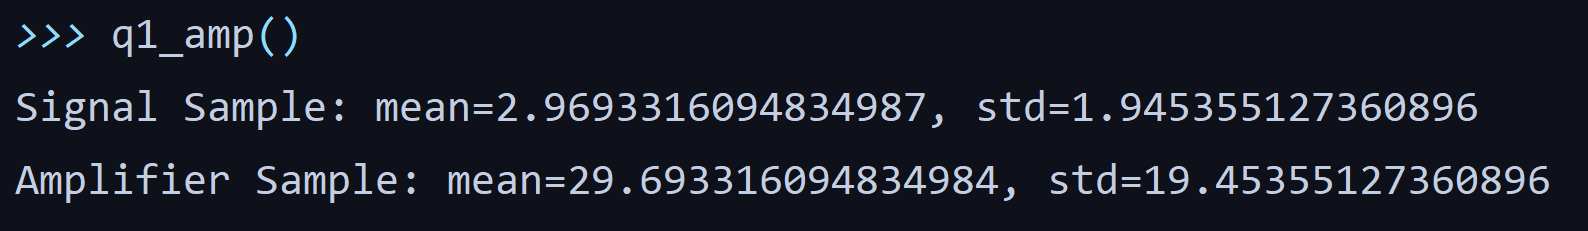
\includegraphics[width=\linewidth]{inc/q1_out.png}
        \item Averaged Measurements \\
        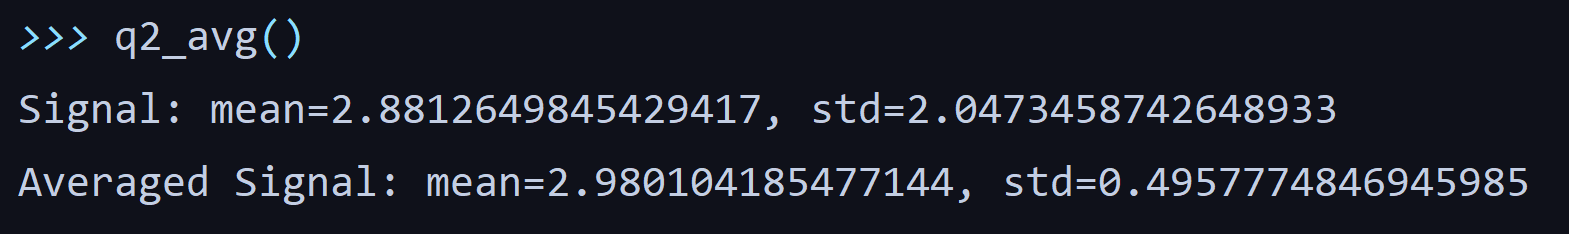
\includegraphics[width=\linewidth]{inc/q2_out.png}
        \item Covariance and Correlation \\
        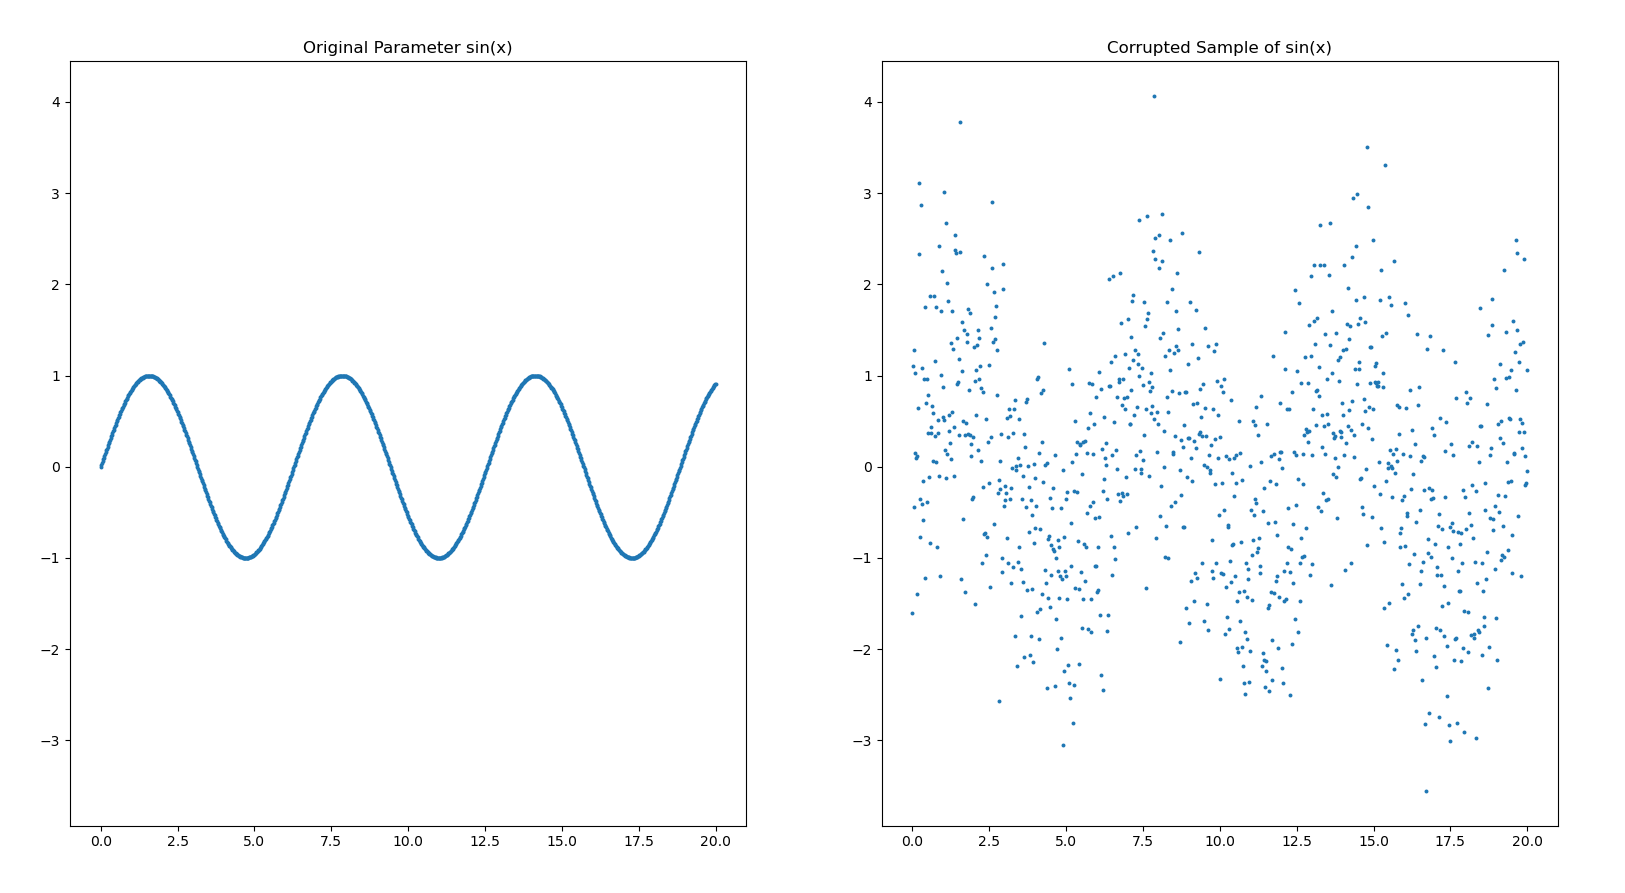
\includegraphics[width=\linewidth]{inc/q3_plot.png} \\
        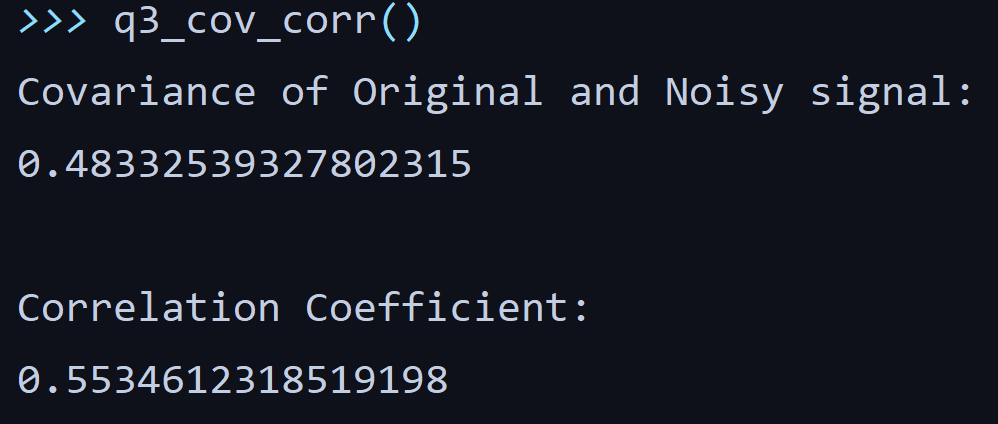
\includegraphics[width=0.5\linewidth]{inc/q3_out.png}
        \item Combined Uncertainty \\
        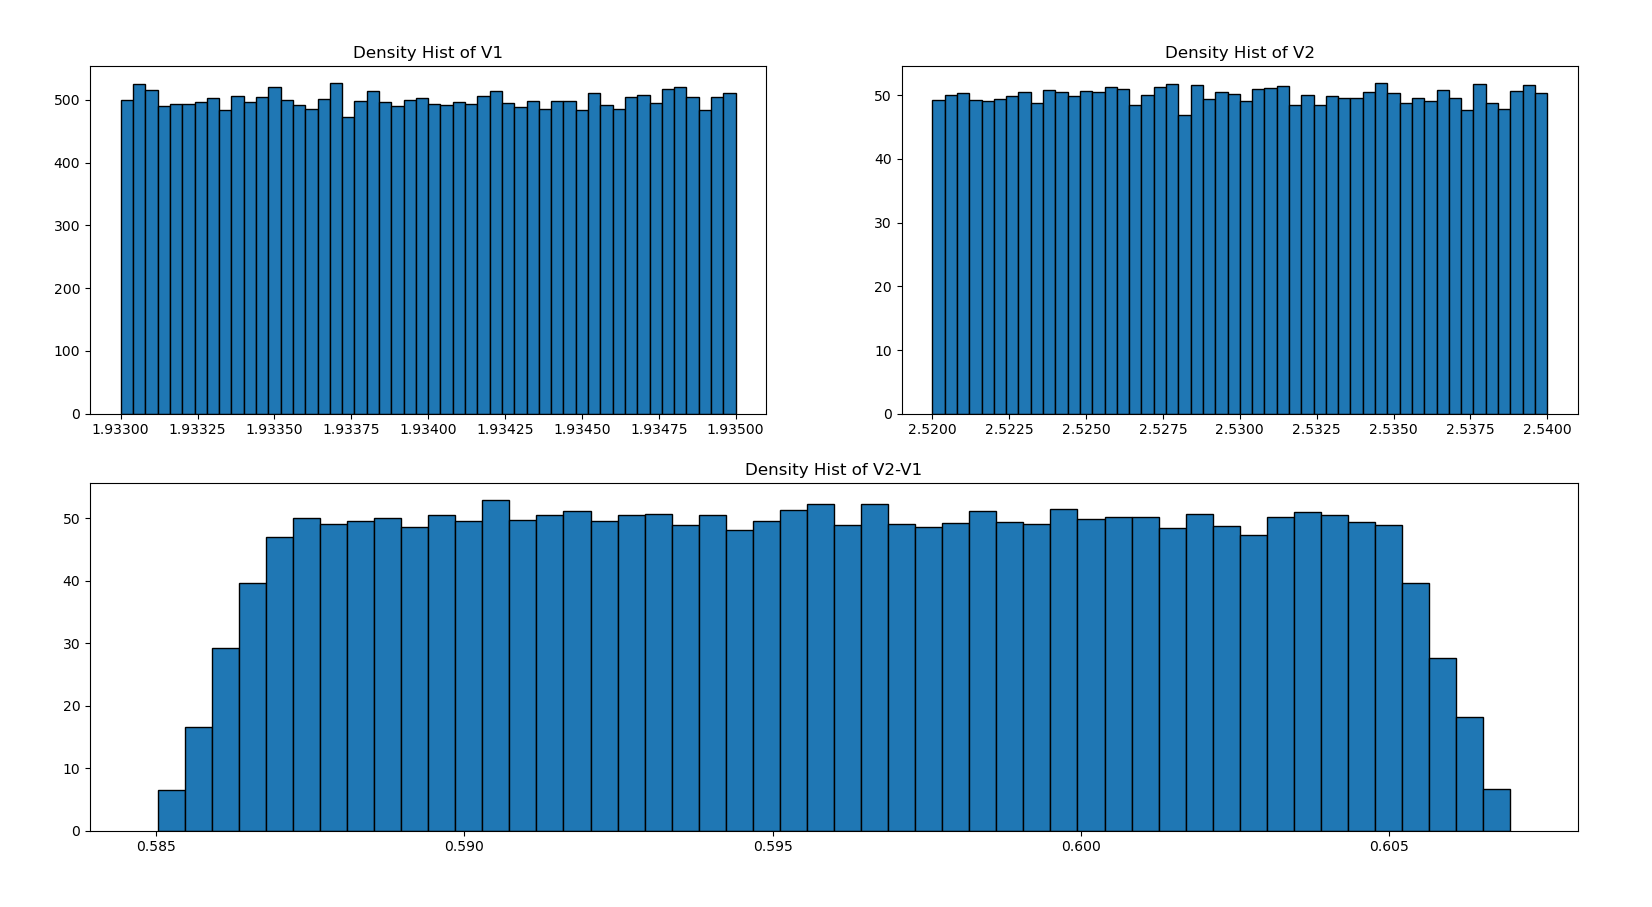
\includegraphics[width=\linewidth]{inc/q4_plot.png} \\
        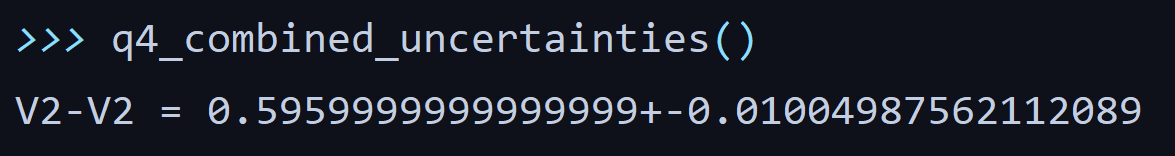
\includegraphics[width=\linewidth]{inc/q4_out.png}
\end{enumerate}

\newpage
\section*{Appendix}
\inputpython{../py/lab2.py}{1}{100}

\end{document}